%%%%%%%%%%%%%%%%%%%%%%%%%%%%%%%%%%%%%%%%%
% Beamer Presentation
% LaTeX Template
% Version 1.0 (10/11/12)
%
% This template has been downloaded from:
% http://www.LaTeXTemplates.com
%
% License:
% CC BY-NC-SA 3.0 (http://creativecommons.org/licenses/by-nc-sa/3.0/)
%
%%%%%%%%%%%%%%%%%%%%%%%%%%%%%%%%%%%%%%%%%

%----------------------------------------------------------------------------------------
%	PACKAGES AND THEMES
%----------------------------------------------------------------------------------------

\documentclass{beamer}

\mode<presentation> {

% The Beamer class comes with a number of default slide themes
% which change the colors and layouts of slides. Below this is a list
% of all the themes, uncomment each in turn to see what they look like.

%\usetheme{default}
%\usetheme{AnnArbor}
%\usetheme{Antibes}
%\usetheme{Bergen}
%\usetheme{Berkeley}
%\usetheme{Berlin}
%\usetheme{Boadilla}
 \usetheme{CambridgeUS}
%\usetheme{Copenhagen}
%\usetheme{Darmstadt}
%\usetheme{Dresden}
%\usetheme{Frankfurt}
%\usetheme{Goettingen}
%\usetheme{Hannover}
%\usetheme{Ilmenau}
%\usetheme{JuanLesPins}
%\usetheme{Luebeck}
%\usetheme{Madrid}
%\usetheme{Malmoe}
%\usetheme{Marburg}
%\usetheme{Montpellier}
%\usetheme{PaloAlto}
%\usetheme{Pittsburgh}
%\usetheme{Rochester}
%\usetheme{Singapore}
%\usetheme{Szeged}
%\usetheme{Warsaw}

% As well as themes, the Beamer class has a number of color themes
% for any slide theme. Uncomment each of these in turn to see how it
% changes the colors of your current slide theme.

%\usecolortheme{albatross}
%\usecolortheme{beaver}
%\usecolortheme{beetle}
%\usecolortheme{crane}
%\usecolortheme{dolphin}
%\usecolortheme{dove}
%\usecolortheme{fly}
%\usecolortheme{lily}
%\usecolortheme{orchid}
%\usecolortheme{rose}
%\usecolortheme{seagull}
%\usecolortheme{seahorse}
%\usecolortheme{whale}
%\usecolortheme{wolverine}

%\setbeamertemplate{footline} % To remove the footer line in all slides uncomment this line
%\setbeamertemplate{footline}[page number] % To replace the footer line in all slides with a simple slide count uncomment this line

%\setbeamertemplate{navigation symbols}{} % To remove the navigation symbols from the bottom of all slides uncomment this line
}

\usepackage{graphicx} % Allows including images
\usepackage{booktabs} % Allows the use of \toprule, \midrule and \bottomrule in tables
\usepackage{dsfont}

% Wenzhen's part needs extra packages
\usepackage{subfig}
\usepackage{multicol}
\usepackage{ amssymb }
%\usepackage{physics}
%\usepackage{sfmath}
\usepackage{amsmath,amsfonts,amsthm,bm} % Math packages
\DeclareMathAlphabet{\mathbbm}{U}{bbm}{m}{n}
%----------------------------------------------------------------------------------------
%	TITLE PAGE
%----------------------------------------------------------------------------------------

\title[Logistic Regression]{Logistic Regression} % The short title appears at the bottom of every slide, the full title is only on the title page

\author{Wenzhen Zhu, Sayantan Bhadra, Cancan Li, Charlie Wu, Chih Yun Pai} % Your name
\institute[WUSTL] % Your institution as it will appear on the bottom of every slide, may be shorthand to save space
{
Washington University in St. Louis \\ % Your institution for the title page
\medskip
\textit{CSE 543T} % Class Number
}
\date{\today} % Date, can be changed to a custom date

\begin{document}

\begin{frame}
\titlepage % Print the title page as the first slide
\end{frame}

\begin{frame}
\frametitle{Overview} % Table of contents slide, comment this block out to remove it
\tableofcontents % Throughout your presentation, if you choose to use \section{} and \subsection{} commands, these will automatically be printed on this slide as an overview of your presentation
\end{frame}
%----------------------------------------------------------------------------------------
%	PRESENTATION SLIDES Section 2
%----------------------------------------------------------------------------------------
\section{Logistic Regression} 

%------------------------------------------------
\subsection{Iris Flower}
\begin{frame}
\frametitle{Fisher's Iris}
The data set consists of 50 samples from each of three 
species of iris flowers.  Four features were measured from each
sample, they are the length and the width of sepal and petal. This data set is often used
to demonstrate classification techniques and discriminant analysis.

\begin{figure}[htbp] \centering \subfloat[setosa]{
    \label{fig:subfig_a}
    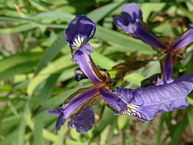
\includegraphics[scale=.4]{graphics/setosa}
}
\hspace{20pt} \subfloat[versicolor]{
    \label{fig:subfig_b}
    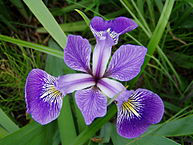
\includegraphics[scale=.4]{graphics/versicolor}
}
\hspace{20pt} \subfloat[virginica]{
    \label{fig:subfig_c}
    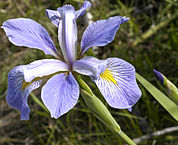
\includegraphics[scale=.4]{graphics/virginica}
}
\caption{Iris } \end{figure}
\end{frame}

%------------------------------------------------
\begin{frame}
\frametitle{Fisher's Iris}
Four features were measured from each
sample, they are the length and the width of sepal and petal.
\begin{figure}[htbp]
\centering
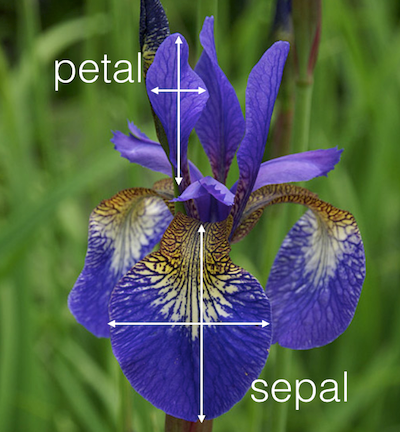
\includegraphics[scale=.35]{graphics/iris_feature} \caption{Features}
\label{fig:Features}
\end{figure}
\end{frame}
%------------------------------------------------
\begin{frame}
\frametitle{Sample Data}

\begin{table}
\begin{tabular}{lllll}
\hline
\textbf{Sepal Length} & \textbf{ Sepal Width } & \textbf{Petal Length} & \textbf{Petal Width} & \textbf{Species}\\
\hline
5.8 & 4.0 & 1.2 & 0.2 & setosa\\
6.4 & 2.8 & 5.6 & 2.1 & virginica\\
6.7 & 3.1 & 5.6 & 2.4 & virginica \\
\hline
\end{tabular}
\caption{Fisher's Iris Dataset Sample}
\end{table}

\begin{figure}[htbp]
\centering
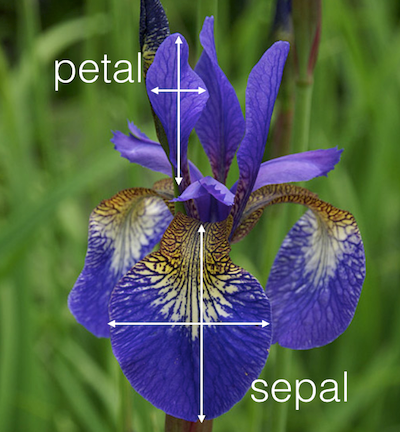
\includegraphics[scale=.23]{graphics/iris_feature} \caption{Features}
\end{figure}


\end{frame}
%------------------------------------------------
\begin{frame}
\frametitle{Visualization of Iris Dataset}
\begin{figure}[t]
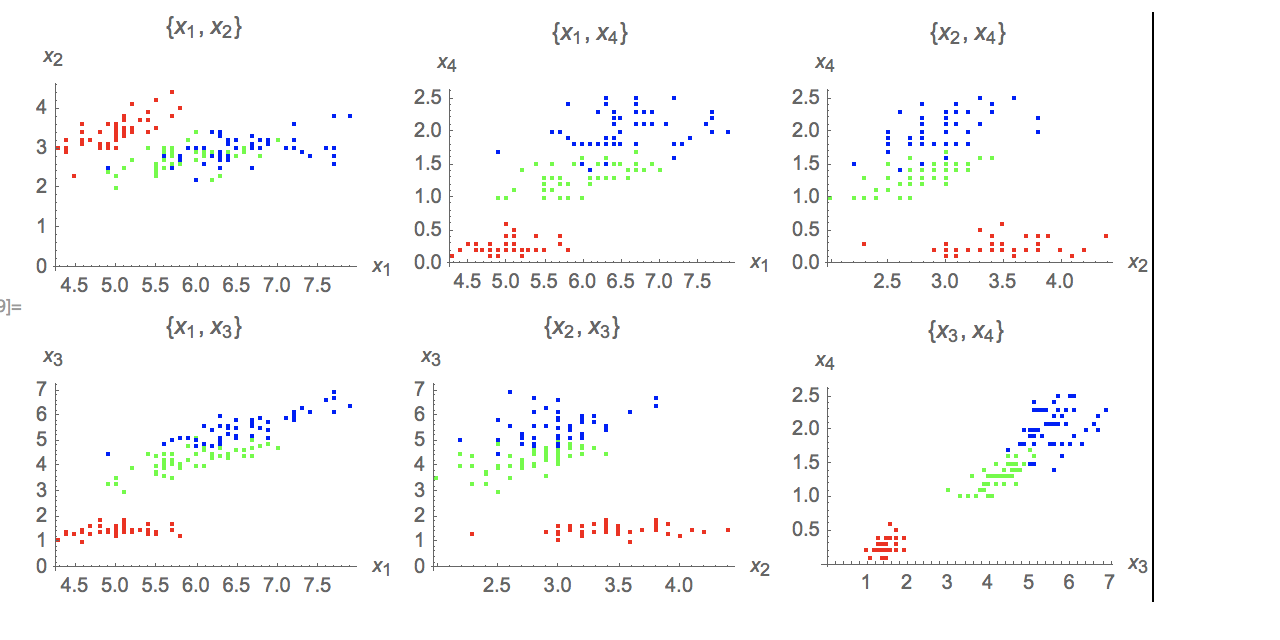
\includegraphics[scale=0.5]{graphics/feature_vis}
\centering
\end{figure}
\end{frame}
%------------------------------------------------
\begin{frame}
\frametitle{}
\[\text{Let's start from binary classification y $\in $ $\{$0, 1$\}$}\]

\[\text{y $\in $ $\{$0, 1$\}$   where 0 $\to $ versicolor 1$\to $ virginica}\]
\[	
	\mathbf{x} = (x_ 1, x_ 2) \
		where \ x_1 = \text{sepal width}, x_2 = \text{petal width}\]
\end{frame}
%------------------------------------------------
\subsection{Sigmoid Function}
\begin{frame}
\frametitle{Sigmoid Function}
\[p(x)=\frac{1}{1+e^{-x}}\]
\begin{figure}[t]
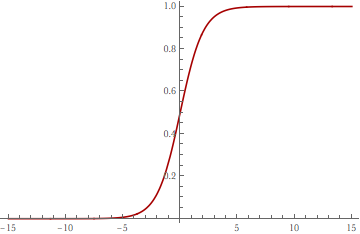
\includegraphics[width=5cm]{graphics/1d-sigmoid}
\centering
\end{figure}
\end{frame}
%------------------------------------------------
\begin{frame}
\begin{multicols}{2} % 2 columns
\begin{figure}[t]
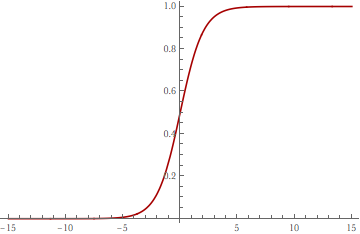
\includegraphics[width=5cm]{graphics/1d-sigmoid}
\centering
\end{figure}
\columnbreak  % seperate
In this example, you can think 
\[ \bm{\theta} = (\theta_{0}, \theta_{1}) \ and \ \mathbf{x} = (1, x)\]
therefore, 
\[p(\mathbf{x}) =  \frac{1}{1+e^{- ( \theta_{0} +  \theta_{1} \cdot  x )}} \]
\\
\end{multicols}

\begin{multicols}{2}
\[p(x) \geq \frac{1}{2}  \Rightarrow class 1\]
\[p(x)<\frac{1}{2}  \Rightarrow class 0\]
\columnbreak 
\[p(\mathbf{x})=P(y=1|\mathbf{x}) = \frac{1}{1+e^{-\bm{\theta} ^\intercal\mathbf{x}}}\]
\[1-p(\mathbf{x})=P(y=0|\mathbf{x}) = \frac{e^{-\bm{\theta} ^\intercal \mathbf{x}}} {1+e^{-\bm{\theta}^\intercal \mathbf{x}}} \]
\end{multicols}

\end{frame}
%------------------------------------------------ 
\begin{frame}
\begin{centering}
\begin{aligned}
class 1 &\Leftrightarrow p(\mathbf{x}) = \frac{1}{1+e^{-\bm{\theta} ^\intercal \mathbf{x}}} > \frac{1}{2} \\
&\Leftrightarrow e^ {-\bm{\theta} ^\intercal \mathbf{x}} > 1\\
&\Leftrightarrow \bm{\theta} ^\intercal \mathbf{x} > 0\\
\end{aligned}
\\
\begin{aligned}
class 0 &\Leftrightarrow p(\mathbf{x}) = \frac{1}{1+e^{-\bm{\theta} ^\intercal \mathbf{x}}} < \frac{1}{2} \\
&\Leftrightarrow e^ {-\bm{\theta} ^\intercal \mathbf{x}} < 1\\
&\Leftrightarrow \bm{\theta} ^\intercal \mathbf{x} < 0\\
\end{aligned}

\end{centering}
%\[p(\mathbf{x}) = \frac{1}{1+e^{-\bm{\theta} ^\intercal \mathbf{x}}} \geq \frac{1}{2} \Leftrightarrow \bm{\theta} ^\intercal \mathbf{x} > 0 \Rightarrow class 1\]
%\[p(\mathbf{x}) = \frac{1}{1+e^{-\bm{\theta} ^\intercal \mathbf{x}}} <\frac{1}{2}  \Leftrightarrow \bm{\theta} ^\intercal \mathbf{x} < 0 \Rightarrow class 0\]
\\
\begin{block}{Conclusion}
\begin{itemize}
\item Logistic regression gives us a \textbf{linear classifier}. \\
\item $\bm{\theta}  ^\intercal \mathbf{x} = 0$ is \textbf{decision boundary}. 
\end{itemize}
\end{block}
\end{frame}
%------------------------------------------------
\begin{frame}
3D Visualization \\
See a Mathematica Dynamic Visualization
\end{frame}
%------------------------------------------------
\subsection{Likelihood Function for Logistic Regression}
\begin{frame}
\frametitle{Maximum Likelihood}

% likelihood
\begin{equation}
\begin{aligned}
L(\bm{\theta}) &= \prod_{i=1}^n P(Y = y_{i}  | X = \mathbf{x}_{i}) = \prod_{y_{i} = 0 } (1-p(\mathbf{x}_{i})) \prod_{y_{i} = 1 } (p(\mathbf{x}_{i})) \\
&= \prod_{i=1}^{n} p(\mathbf{x}_{i})^{y_{i}} ^\intercal (1-p(\mathbf{x}_{i}))^{(1-{y_{i}})}
\end{aligned}
\end{equation}

\begin{equation}
\begin{aligned}
l (\bm{\theta}) &=  \log (L(\bm{\theta}) ) = \sum_{i=1}^{n} y_{i} \log(p(\mathbf{x}_{i}) + (1-y_{i}) \log(1-p(\mathbf{x}_{i})) \\
&= \sum_{y_{i} = 0 } \log (1-h(\mathbf{x}_{i})) + \sum_{y_{i} = 1} \log (h(\mathbf{x}_{i})) \\
\end{aligned}
\end{equation}
Since $f(x) = log(x)$ is a monotonically increasing function, maximizing $L(\bm{\theta})$ is equivalent as maximizing $l(\bm{\theta})$
\end{frame}
%------------------------------------------------
\begin{frame}
\frametitle{Maximum Likelihood Estimation}
Set derivatives equal to zero, then solve, we will find the maximum likelihood.
Let $p(x) = g(\bm{\theta} ^\intercal \mathbf{x}) = \frac{1}{1+ e^{-\bm{\theta} ^\intercal \mathbf{x}}}$
\begin{equation}
\begin{aligned}
l'(\bm{\theta}) &= \frac{\partial l}{\partial \bm{\theta}} =\left(y \frac{1}{g(\bm{\theta} ^\intercal \mathbf{x})} - (1-y) \frac{1}{1-g(\bm{\theta} ^\intercal \mathbf{x})}\right) 
\frac{\partial }{\partial \bm{\theta_{j}}} g(\bm{\theta} ^\intercal \mathbf{x}) \\
&= \frac{\partial l}{\partial \bm{\theta}} =\left(y \frac{1}{g(\bm{\theta} ^\intercal \mathbf{x})} - (1-y) \frac{1}{1-g(\bm{\theta} ^\intercal \mathbf{x})}\right) 
g(\bm{\theta} ^\intercal \mathbf{x})(g(\bm{\theta} ^\intercal \mathbf{x})) 
\frac{\partial }{\partial \bm{\theta_{j}}} \bm{\theta} ^\intercal \mathbf{x} \\
&= \left(y(1-g(\bm{\theta} ^\intercal \mathbf{x}) - (1-y) g(\bm{\theta} ^\intercal \mathbf{x}) \right) x_{j} \\
&= (y - p(\mathbf{x}))x_{j}


Solve for $\bm{\theta}$ by setting $l'(\bm{\theta}) =0$

\end{aligned}
\end{equation}
\end{frame}
%------------------------------------------------
\subsection{Logistic Regression with More Than Two Classes}
\begin{frame}
\frametitle{Logistic Regression with More Than Two Classes}
If $Y$ can take on $k$ values, i.e. we have $k$ classes, we can still use logistic regression. The predicted conditional probabilities will be 
\begin{equation}
P(Y = c | X = \mathbf{x}) = \frac{\exp ({\bm{{\theta}^{c}} ^\intercal \mathbf{x}})}{ \sum_{j}^{k} \exp(\bm{{\theta}^{j} }^\intercal \mathbf{x}) }
\end{equation}
\end{frame}


%------------------------------------------------

%----------------------------------------------------------------------------------------
%	PRESENTATION SLIDES Section 5  Application
%----------------------------------------------------------------------------------------
\section{Application} 
%------------------------------------------------
\subsection{MNIST}
\begin{frame}
\frametitle{Logistic Regression on MNIST Dataset}
Let's take a look of a fast prototype..
\begin{figure}[t]

\includegraphics[width=10cm]{graphics/mnist}
\centering
\end{figure}
\end{frame}
%------------------------------------------------
\subsection{CIFAR-10}
\begin{frame}
\frametitle{Logistic Regression on CIFAR-10 Dataset}
CIFAR-10  is an established computer-vision dataset used for object recognition. It consists of 60,000 32x32 color images containing one of 10 object classes, with 6000 images per class. 
Here are the classes in the dataset, as well as 10 random images from each:
\begin{figure}[t]
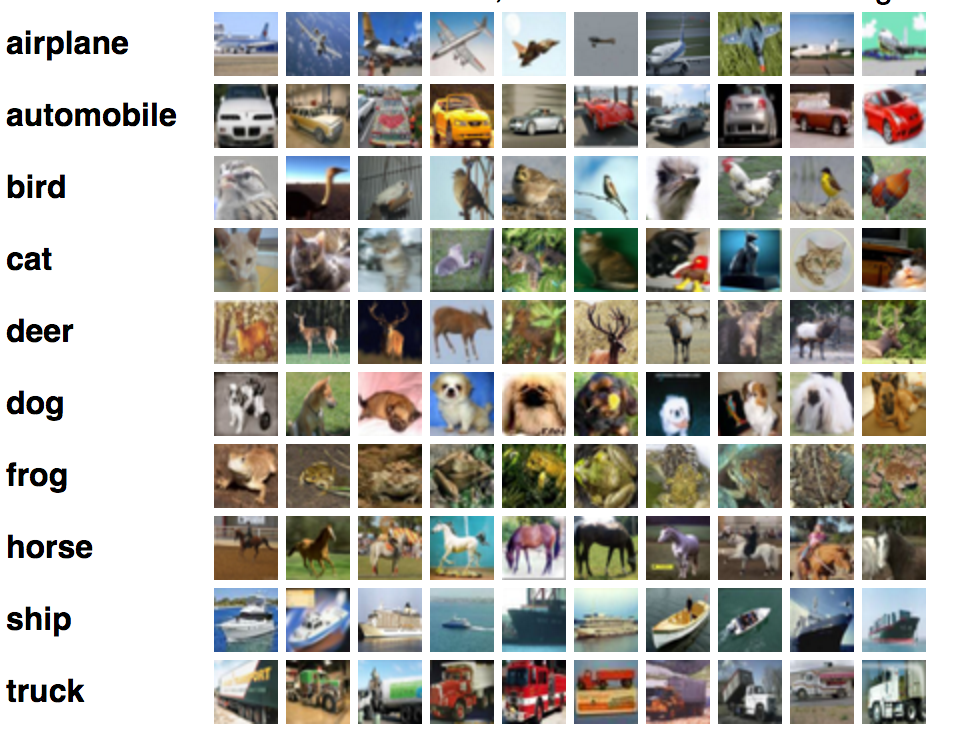
\includegraphics[width=7cm]{graphics/cifar-10}
\centering
\end{figure}
\end{frame}
%------------------------------------------------

%----------------------------------------------------------------------------------------
%	PRESENTATION SLIDES EXTRA
%----------------------------------------------------------------------------------------

\begin{frame}[fragile] % Need to use the fragile option when verbatim is used in the slide
\frametitle{Citation}
An example of the \verb|\cite| command to cite within the presentation:\\~

This statement requires citation \cite{p1}.
\end{frame}

%------------------------------------------------

\begin{frame}
\frametitle{References}
\footnotesize{
\begin{thebibliography}{99} % Beamer does not support BibTeX so references must be inserted manually as below
\bibitem[Smith, 2012]{p1} John Smith (2012)
\newblock Title of the publication
\newblock \emph{Journal Name} 12(3), 45 -- 678.
\end{thebibliography}
}
\end{frame}

%------------------------------------------------

\begin{frame}
\Huge{\centerline{The End}}
\end{frame}

%----------------------------------------------------------------------------------------

\end{document} 